After installing/compiling \biodeg{} as described in Section~\ref{sec:installation}, we are ready to run it. There are 2 ways to run \biodeg{} simulations: 1) using the UI to configure and execute \biodeg{}, or 2) running \biodeg{} directly from the command line and providing simulation parameters via command-line arguments. Moreover, in a hybrid approach, the UI can be used to configure and generate the command for method \#2, which can be useful when you want to configure the simulation only and run it later in another environment like on a super-computer or cluster.

The UI can be run simply by double-clicking on the \verb|BioDeg-UI.exe| in Windows or by executing \verb|./BioDeg-UI| in Linux. For running \biodeg{} directly, one need to execute the following command:
\begin{verbatim}
$ mpirun -n N FreeFem++-mpi core/src/main.edp <command line args>
\end{verbatim}
in which N defines the number of MPI processes to be used. The full list of command-line arguments can be found in Section \hyperref[sec:index]{Index}.

In order to clarify and demonstrate the procedure of performing simulations using \biodeg{}, 2 step-by-step examples are provided in Section~\ref{sec:config}, showing how to configure and run simulations with and without the UI. Moreover, a third example shows how to combine these approaches and use the UI to generate the execution command. The mesh files needed to run these examples can be found in the \verb|demo| directory. Additionally, Section~\ref{sec:postprocess} provides some guidelines on the postprocessing of the  \biodeg{} simulation results. 

\subsection{Configuring the simulation} \label{sec:config}


\subsubsection{Example 1 - degradation of a simple screw}\label{sec:example1}

Let us consider the first example given in the \verb|demo| directory, where we simulate the biodegradation of a small screw. The size of the screw was chosen to be very small intentionally to make the simulation shorter such that the user can see the effect of the degradation much faster. The input mesh file is named \verb|screw.mesh|. For this example, we use the \biodeg{}-UI interface to perform the simulation. 

Let's conduct the first simulation with most of the parameters left with their default values. Run the user interface, and mark \menu[,]{Geometry \& Mesh, Import external mesh}. Then click the browse button in front of the ``File'' box (\menu[,]{Geometry \& Mesh, Import mesh, File}), navigate to the \verb|demo| directory, and select the \verb|screw.mesh| file. The path should be inserted in the ``File'' box. Selecting appropriate label numbers of the external mesh is very crucial in \biodeg{}, so you should always check the labels before importing the mesh. One of the best tools to do this is GMSH, in which you can view the labels of mesh files by opening the mesh and navigating to \menu[,]{Tools, Visibility}. Doing this on the \verb|screw.mesh| shows that the label number of the scaffold is 2 while the medium has a label number of 1 (Fig.~\ref{fig:gmsh_label}). So, we need to switch the default labels by selecting 2 for the scaffold (\menu[,]{Geometry \& Mesh, Import mesh, Scaffold label}) and 1 for the medium (\menu[,]{Geometry \& Mesh, Import mesh, Medium label}).

\begin{figure}[h]
\center 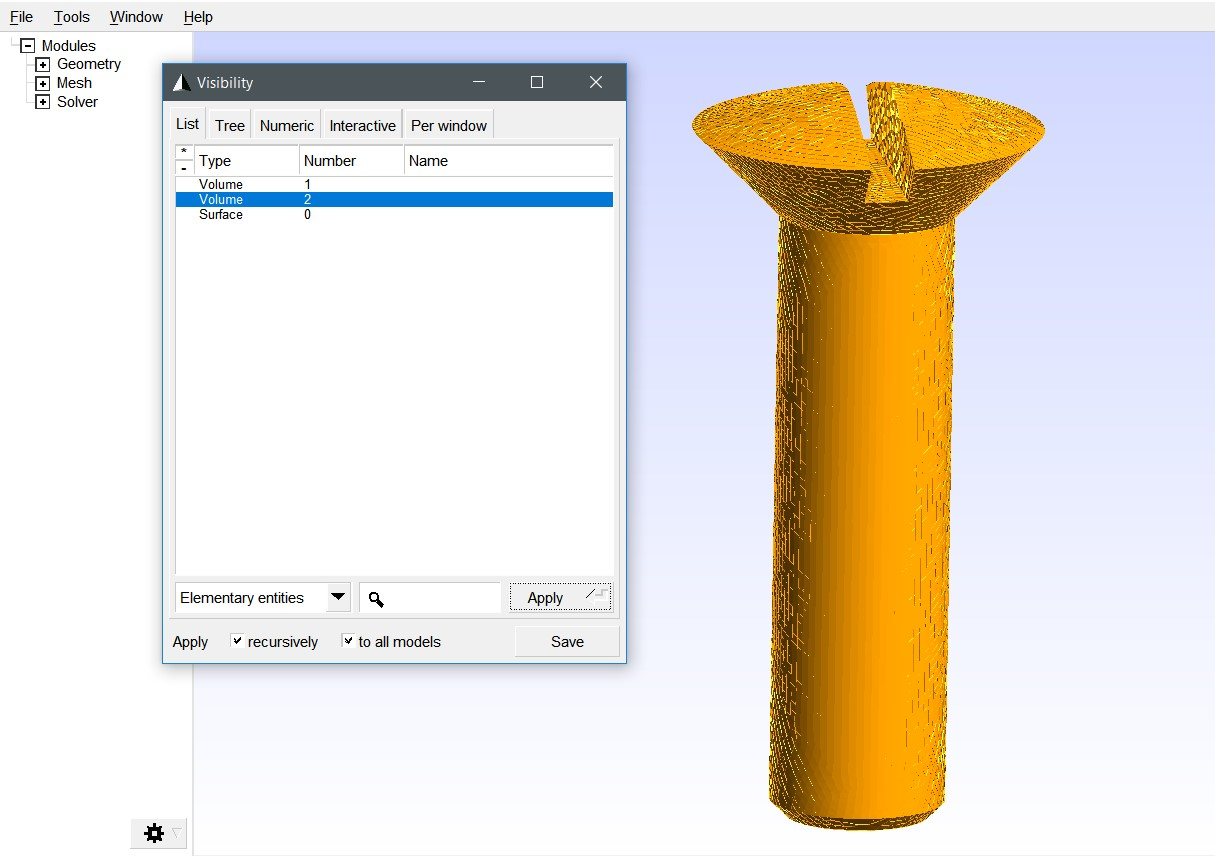
\includegraphics[width=15cm]{gmsh_label}
\caption{Using GMSH to read the labels of the mesh} \label{fig:gmsh_label}
\end{figure}

We need to enable the VTK output if we want to see the graphical output of the simulations. Navigate to \menu[,]{Output, Output options, Write VTK output} and mark it. You should also specify the output directory by clicking on the browse button in front of the ``Output directory'' (\menu[,]{Output, Output options, Output directory}) and select a directory of desire. 

That was all we needed to do to setup a simulation in \biodeg{}, and you can start the simulation by pressing the \menu[,]{Run simulation} button located in the middle of the main window. There are lot more parameters we can deal with (see Section \hyperref[sec:index]{Index}), but the input and output are the most essential ones. 

Although you can start the simulation of this example right now, there is a couple of more things you may want to change:

\begin{itemize}
\item
In \biodeg{}, simulations are by default carried out in parallel using domain decomposition, meaning that the simulation is distributed among available computing nodes. If you are running \biodeg{} on your local machine, you may need to adjust the parallel computing settings. Navigate to \menu[,]{Solver, Parallel computing, Enable parallel computing} and disable it if you don't want to parallelize the simulation. If you want to continue with parallelization enabled (default behavior), you may need to adjust the number of parallel processes to match the number of free CPU cores you have on your machine. You can change it in \menu[,]{Solver, Parallel computing, CPU/MPI cores}. 
\item
The default degradation rate is quite fast, so you may want to decrease it by reducing the diffusion coefficient of the metallic ions (please refer to ``Theory Guide'' if you want to know more about diffusion controls the rate of degradation). The default diffusion rate is the value we have estimated for saline solutions, which leads to a high rate of corrosion. You can apply this by changing the value in \menu[,]{Material \& BCs, Reaction-diffusion properties, Metal ion diffusion coefficient} and reduce it to something like $0.0005$, which is its order when it comes to buffered solutions and simulated body fluids.
\item
The results write interval, implying how frequently you want to store the results, affects the resource consumption (which is the storage in this case) and the quality of the graphical postprocessing. So, you should configure this carefully to keep the balance of quality and resource consumption. The default save interval is $0.25$ hours of simulation time, but you can change it in \menu[,]{Output, Output options, Save results every ... hours}. For this simulation, since the screw geometry is small and degrades very fast, you can reduce this to $0.1$ to be able to see the degradation steps better.
\item
Final simulation time does not affect the simulation progress, but it is always a good practice to adjust it, enabling us to track the progress of the simulation better and avoid wasting resources (both computing power and storage). The default simulation time is 21 hours, but you can reduce it in \menu[,]{Solver, Time control, Final simulation time (hour)}. For this simulation, you can reduce it to 2.
\end{itemize}

After running the simulation (by pressing the \menu[,]{Run simulation} button), you can view the progress of the simulation on the UI, showing you how many steps have been taken and how much material degradation has happened (Fig~\ref{fig:screw_gui}). The UI also shows you the details info of the size of the problem, including the degrees of freedom (DOF) of each equation and the number of elements, as well as the number of DOFs for each sub-domain after mesh partitioning (for parallel computing). 

\begin{figure}[h]
\center 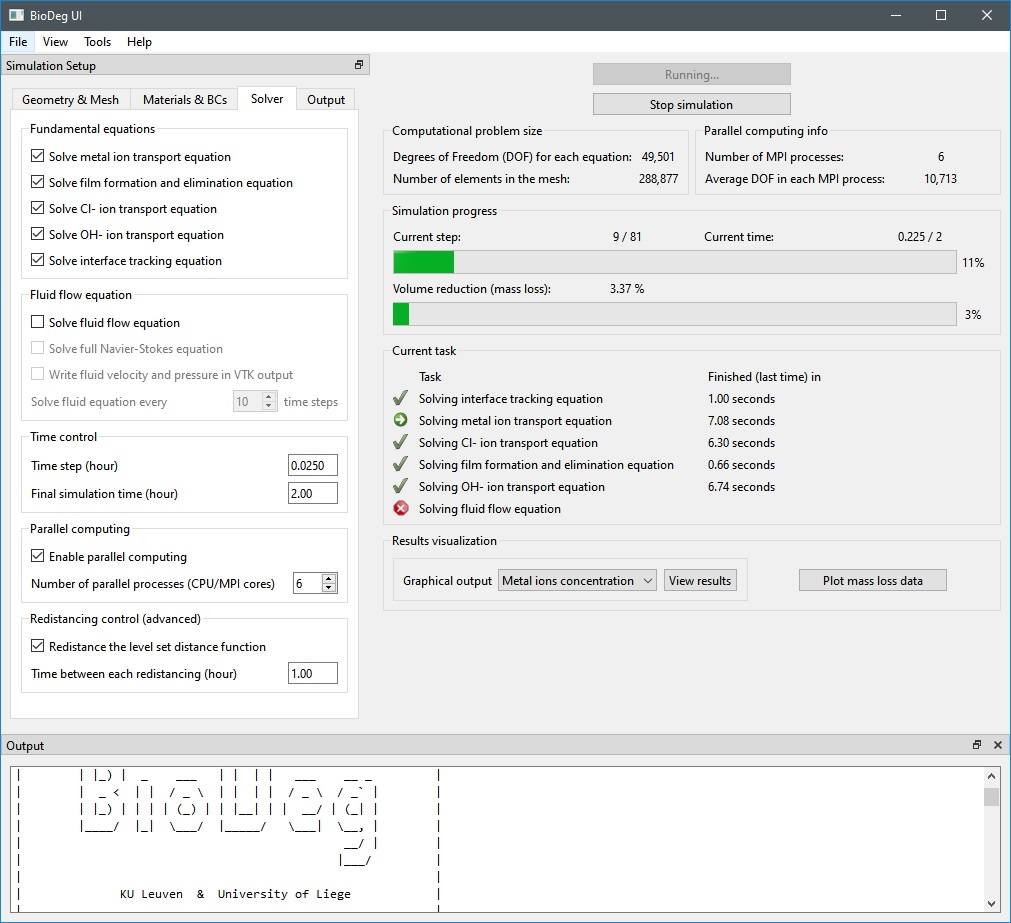
\includegraphics[width=12cm]{screw_gui}
\caption{\biodeg{}-UI running the screw degradation example.} \label{fig:screw_gui}
\end{figure}

Running this simulation leads to the results demonstrated in Fig.~\ref{fig:screw_degradation}, showing how the screw degrades. For more information on how to postprocess the results, please refer to the postprocessing section.

\begin{figure}[h]
\center 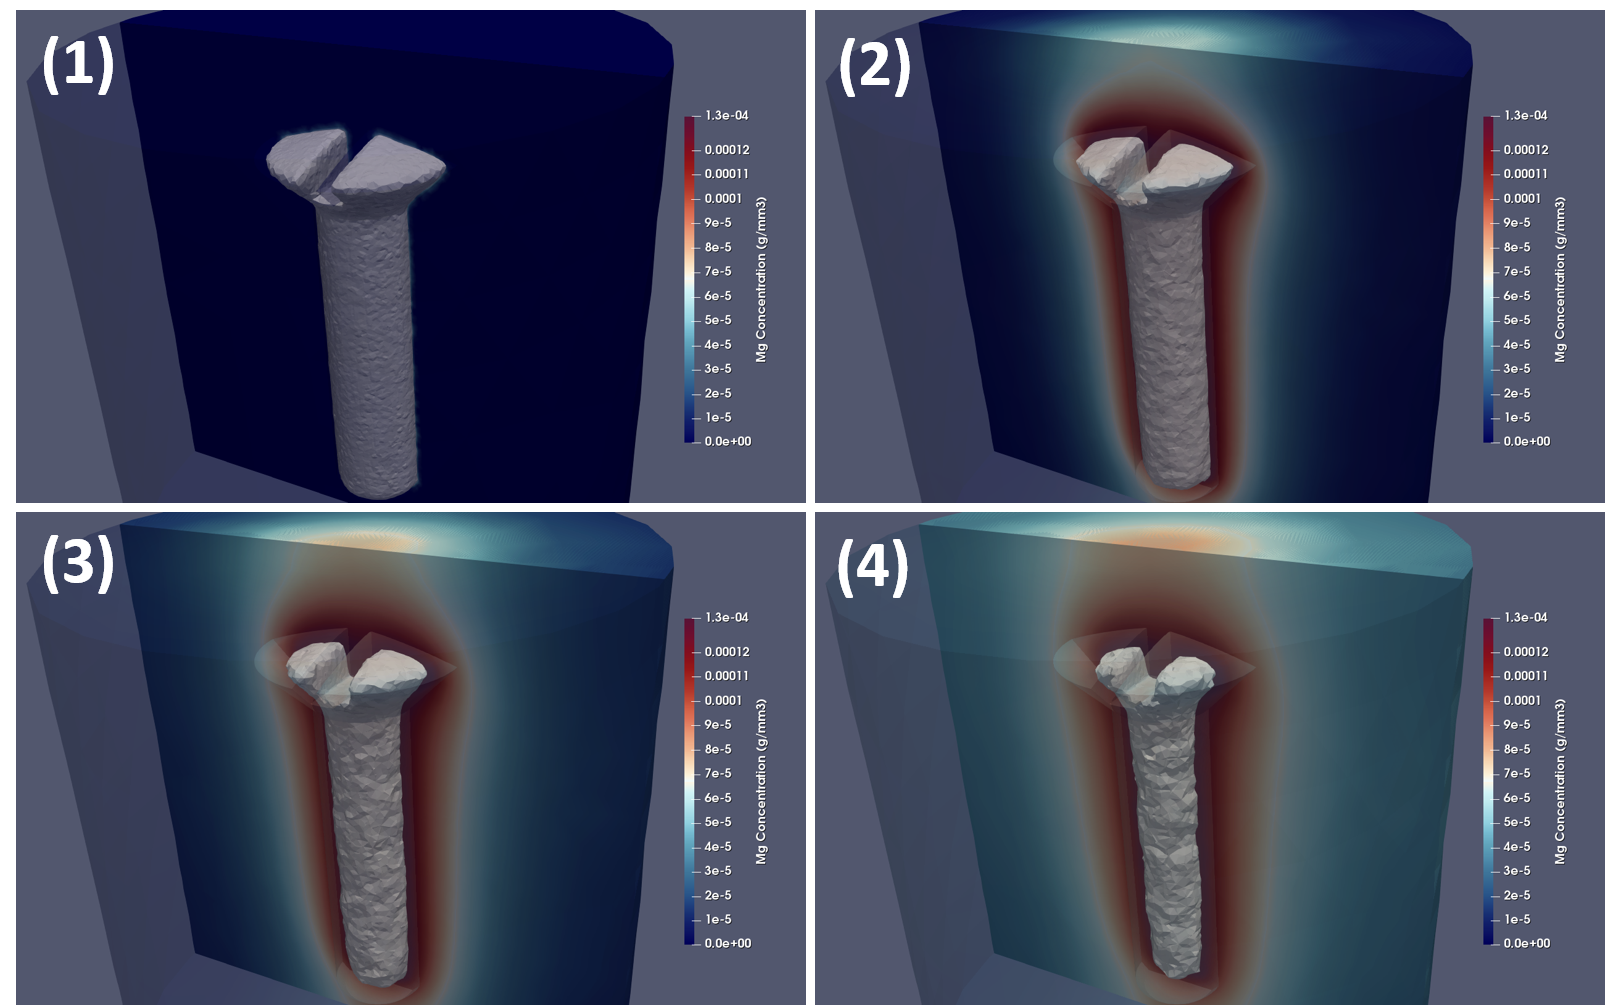
\includegraphics[width=15cm]{screw_degradation}
\caption{Simulation of the biodegradation of a simple screw, showing how the material is released and how the implant degrades.} \label{fig:screw_degradation}
\end{figure}


\subsubsection{Example 2 - degradation of a helical shape (Biomech logo)}\label{sec:example2}

In the second example, we want to run a heavier biodegradation simulation (with $\num{1484412}$ elements and a DOF of $\num{254157}$ for each equation), so let's do it by calling \biodeg{} directly on the command line. This approach can be taken on remote clusters and HPC environments to run \biodeg{} on hundreds or thousands of computing nodes. 

The model in this example has a helical shape, which is actually the logo of the lab in which \biodeg{} has been developed. The input mesh file is called \verb|biomech_logo.mesh| and is located in the \verb|demo| directory. Similar to the previous example, we try to use the default value of parameters and only change the crucial ones. You should notice that the default value of parameters might be different between the core \biodeg{} and the UI, so it's always better to define them explicitly in the execution command. The default values of parameters can be checked in Section  \hyperref[sec:index]{Index}.

The main file of the \biodeg{} code is called \verb|main.edp|, and since it's a parallel code, we should run it with the \verb|mpiexec| command. So, calling the code with all the default parameters on 6 MPI cores can be done like this:
\begin{verbatim}
$ mpiexec -n 6 FreeFem++-mpi core/src/main.edp -v 0
\end{verbatim}

The \verb|-v 0| is added to suppress the messages that FreeFEM writes to the terminal, and it's recommended to include it on any call you make to \biodeg{}. Calling \biodeg{} like this does nothing for us, so let's complete the command by adding more configuration to it (remember that boolean values are passed by their integer equivalents, 0 for false and 1 for true):

\begin{itemize}
\item
Turn off the fluid flow simulation and ignore the convection effect: \verb|-solve_fluid 0|
\item
Indicate that we want to import an external mesh: \verb|-import_mesh 1|
\item
Specify the name of the mesh, located in the \verb|demo| directory: \verb|-mesh_file "demo/biomech_logo.mesh"|
\item 
Specify the labels of different regions, which are crucial parameters as discussed in previous example (Section~\ref{sec:example1}): \verb|-label_scaffold 3 -label_medium 4|
\item
You can lower the degradation rate a little bit if you like. You may run the simulation several times and see the effect of this parameter in action: \verb|-d_mg 0.005|
\end{itemize}

Adding all the above arguments forms the final execution command to run:
\begin{verbatim}
$ mpiexec -n 6 FreeFem++-mpi core/src/main.edp -v 0 -solve_fluid 0 -import_mesh 1 
-mesh_file "demo/biomech_logo.mesh" -label_scaffold 3 -label_medium 4 -d_mg 0.005
\end{verbatim}

The above command executes \biodeg{}, which writes its output to the terminal (Fig~\ref{fig:logo_terminal}) and stores the simulation results to the default directory called \verb|output| (make sure it exists before calling \biodeg{}). 

\begin{figure}[h]
\center 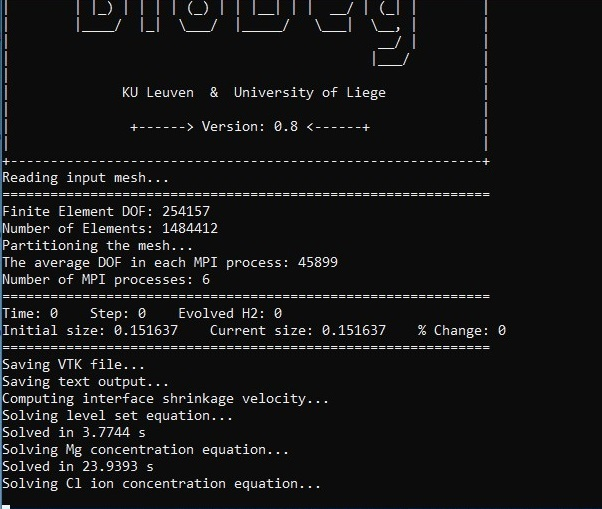
\includegraphics[width=10cm]{logo_terminal}
\caption{Output of \biodeg{} code for the logo example.} \label{fig:logo_terminal}
\end{figure}

The output of this simulation is shown in Fig~\ref{fig:logo_degradation}, which is postprocessed using the NVIDIA IndeX. Please refer to the postprocessing section to see how to do it.

\begin{figure}[h]
\center 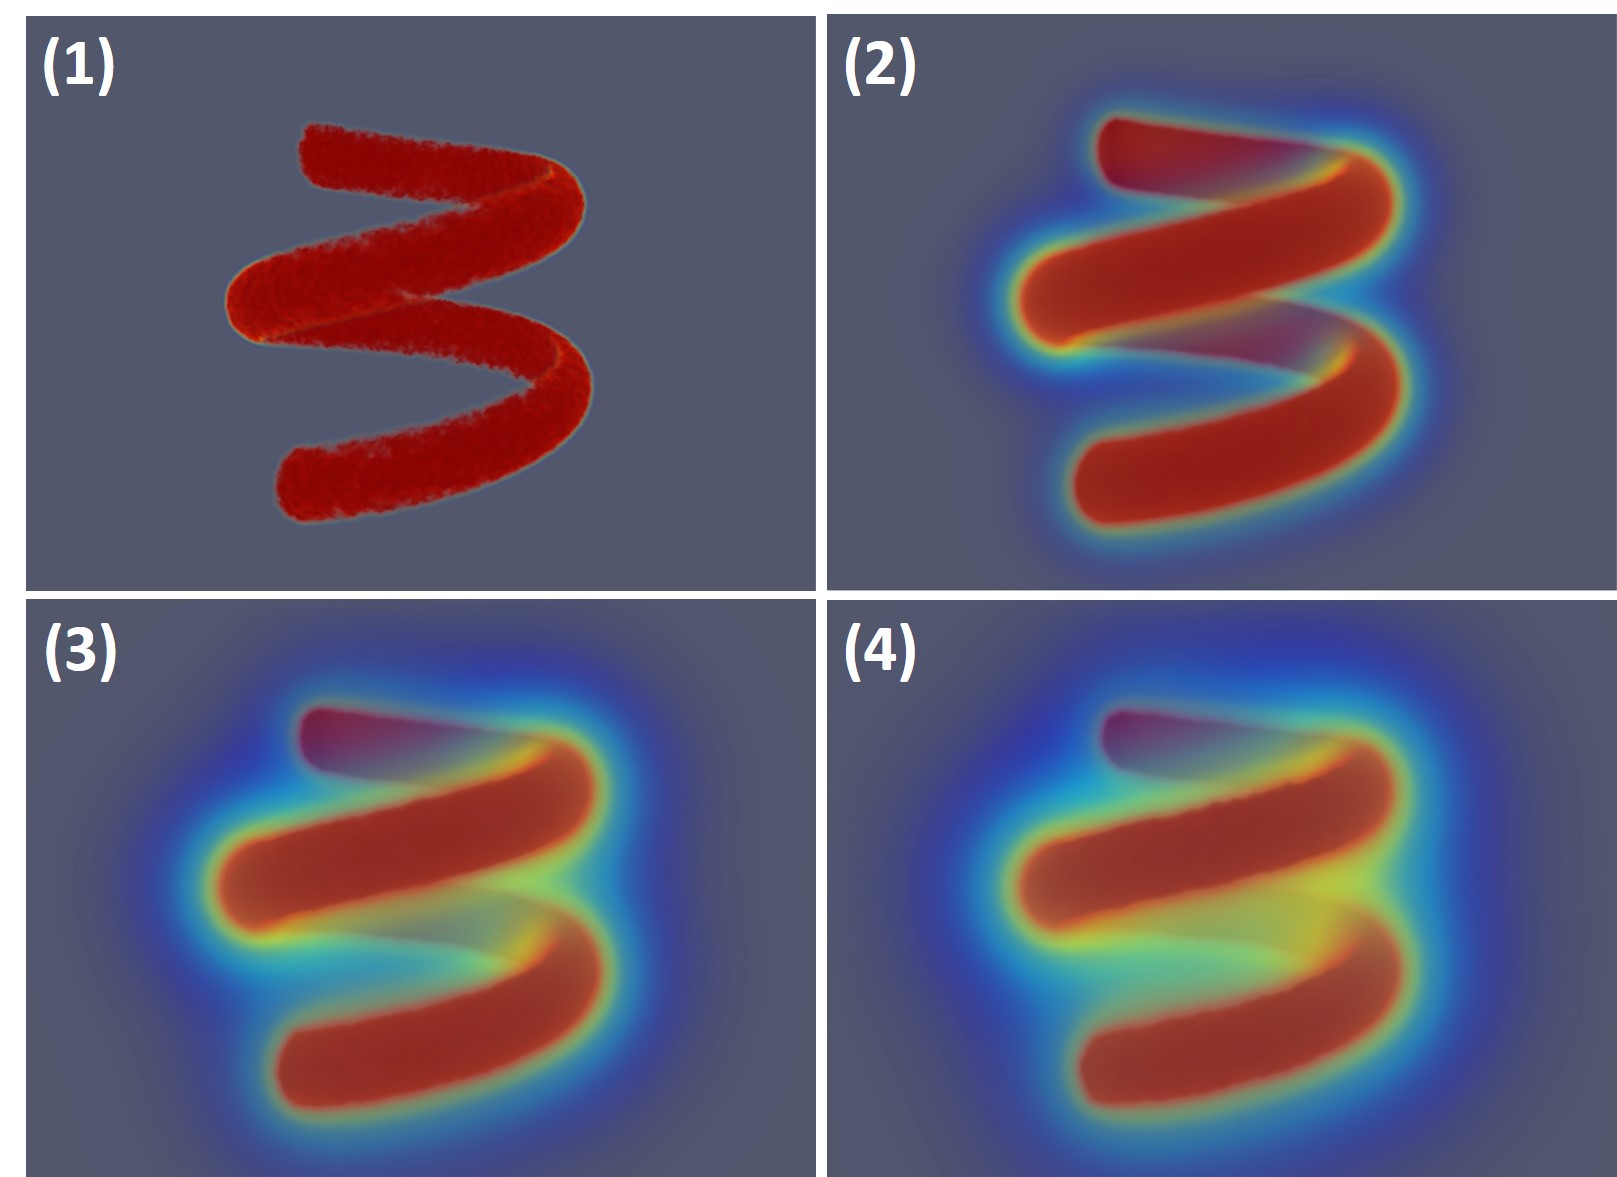
\includegraphics[width=12cm]{logo_degradation}
\caption{Simulation result of the logo example.} \label{fig:logo_degradation}
\end{figure}

\subsubsection{Example 3 - biodegradation of a cuboid}\label{sec:example3}

The aim of this example is to show how one can combine the approaches taken in the last two examples and use the UI to generate the execution command so that it can be used to run the model in another environment from the command line. The idea is simple: \biodeg{}-UI writes the run command and the output of the core model in the ``Output'' panel, so we can have the execution command if we setup the simulation, run it, stop it immediately, and have a look at the ``Output'' panel.

For demonstrating this, we simulate the degradation of a cuboid inside a cubic container. The mesh file is called \verb|cuboid.mesh|, which has $\num{830808}$ elements. The mesh labels for scaffold and medium are the same as the default values on the \biodeg{}-UI (1 for scaffold and 2 for medium), so we don't need to change them. The setup will be straightforward since we just need to adjust the input and output, but the UI will generate a command with a full list of arguments, making it easy to modify it later if required.

Start the UI,
make sure \menu[,]{Geometry \& Mesh, Import external mesh} is checked, click the browse button in front of the ``File'' box (\menu[,]{Geometry \& Mesh, Import mesh, File}), navigate to the \verb|demo| directory, and select the \verb|cuboid.mesh| file. Since we don't want to change anything else, go directory to the output settings, mark
 \menu[,]{Output, Output options, Write VTK output} (since we want to have graphical output for postprocessing), and specify the output directory by clicking on the browse button in front of the ``Output directory'' (\menu[,]{Output, Output options, Output directory}) and select a directory of desire. 
 
As the setup is over, we are ready to run the simulation. Click the \menu[,]{Run simulation} button, wait a moment for the command to appear in the ``Output'' panel (written  like \verb|Executing: <command>|), and then click \menu[,]{Stop simulation}. You can now copy the command from the ``Output'' panel by selecting it, right-clicking on it, and choosing \verb|Copy|. For this sample case, the command looks like this:

\begin{verbatim}
$ mpiexec -n 3 FreeFem++-mpi core/src/main.edp -v 0 -import_mesh 1 
-mesh_file "/home/mojtaba/BioDeg/demo/cuboid.mesh" -label_scaffold 1 -label_medium 2 
-refine_initial_mesh 0  -material_density 0.001735 -film_density 0.002344 
-material_satur 0.000134 -material_eps 0.55 -material_tau 1 -k1 7 -k2 1e+10 -d_mg 0.05 
-d_cl 0.05 -d_oh 25 -initial_cl 5.17e-06 -initial_oh 1e-07 -solve_mg 1 -solve_film 1 
-solve_cl 1 -solve_oh 1 -solve_ls 1 -time_step 0.025 -final_time 21 -do_redistance 1  
-redistance_time 1 -solve_fluid 0 -write_fluid_output 0 -text_output_file 
"/home/mojtaba/BioDeg/cuboid_output/output.txt" -write_vtk 1 -vtk_output_name 
"/home/mojtaba/BioDeg/cuboid_output/output" -save_last_state 0 -save_each 0.25 
-output_per_area 0 -save_multiplier 1 -export_scaffold 0  -save_initial_mesh 0 
-save_initial_partitioned_mesh 0
\end{verbatim}

More details of these parameters can be found in Section \hyperref[sec:index]{Index}. You can always omit the parameters with the default value, resulting in a command like the one we made in the second example (Section~\ref{sec:example2}).

\subsection{Postprocessing of the results using ParaView} \label{sec:postprocess}

Although the \biodeg{}-UI provides some basic postprocessing features such as the total amount of mass loss (via clicking on \menu[,]{Plot mass loss data} which reads the output text file) and a couple of ParaView templates (via selecting one of the variables on \menu[,]{Graphical output} and clicking \menu[,]{View results}), it can always  be beneficial to visualize the results the way you want. Doing this enables you to reproduce the demonstration you see in Figs.~\ref{fig:screw_degradation} and \ref{fig:logo_degradation} as well as any plot output you want, such as plotting variables over a line.

The details of the postprocessing steps of \biodeg{} results are discussed in the following YouTube videos, describing how to use ParaView to visualize the degrading scaffold beside plotting other output variables such as film formation and pH changes:

\begin{itemize}
\item 
\url{https://www.youtube.com/watch?v=yeBPGwP3L80&ab_channel=TuxRiders}
\item
\url{https://www.youtube.com/watch?v=Sz-eBML2pxs&ab_channel=TuxRiders}
\end{itemize}

The following video gives you an idea of how to plot the values of different variables over a line and how to do some quantitative analysis on the results:

\begin{itemize}
\item 
\url{https://www.youtube.com/watch?v=tGi-jk2UE2U&ab_channel=TuxRiders}
\end{itemize}

For visualizing the fluid flow, more advanced techniques should be used. The following videos demonstrate how to visualize the fluid field around a degrading object simulated by \biodeg{}:

\begin{itemize}
\item
\url{https://www.youtube.com/watch?v=CByh84hOslU&ab_channel=TuxRiders}
\item
\url{https://www.youtube.com/watch?v=Xzwe94bvGJI&ab_channel=TuxRiders}
\end{itemize}